% roll no 65 KRISHNENDU P U

\textbf{\textcolor{LightMagenta}{Discuss the issues involved in decision tree learning. (May 2019) \hfill 5 marks}}
\\[5pt]

Learning a tree that classifies the training data perfectly may not lead to the tree with the best generalization performance. Training error no longer  provides  a good estimate of how  well the tree will perform on previously  unseen  records  The following are the practical issues of decision tree learning:

i)	\textcolor{purple}{\underline{Overfitting}}: H more complex than C or f

 Overfitting results in	decision trees that	are more	complex	than necessary.Too many branches, some may reflect anomalies due t outliers. It creates poor accuracy for unseen samples.noise or outliers. It creates poor accuracy for unseen samples.
 A hypothesis h is said to overfit the training data if	there is another hypothesis, h’, such that h has smaller error than h’ on the training data but h has larger error on the test data than h’.\\
 
\textcolor{ReddishRose}{Two cases of overfitting:}\\
When there is noise in the data or when the number of training examples are too small. In these cases the algorithm can produce trees that overfit the training examples\\
 
i)	Overfitting due to noise in the training data.

\graphicspath{ {./} }
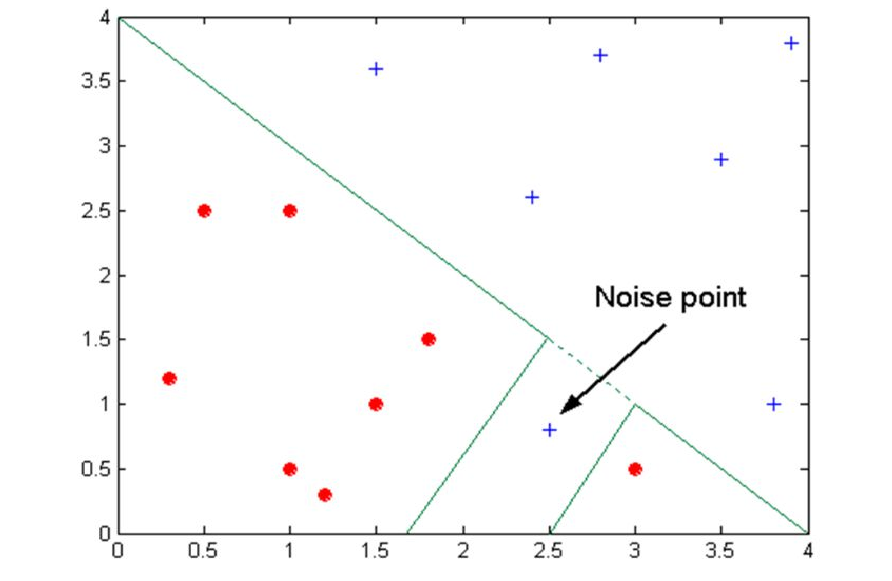
\includegraphics[width=0.5\textwidth]{Images/A27_img1.png}\\


Figure shows that decision boundary is distorted by noise point.\\
ii)	Overfitting due to Insufficient Examples (sample is too small)
Lack of data points  makes it difficult to predict correctly the class labels of  that region
 
\graphicspath{ {./} }
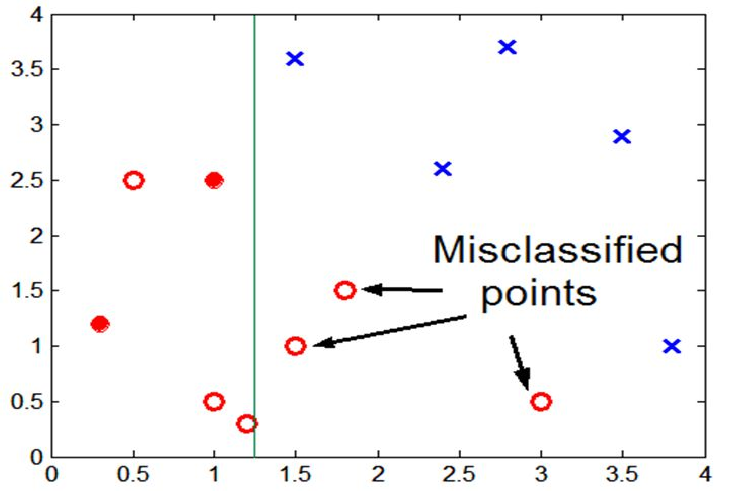
\includegraphics[width=0.5\textwidth]{Images/A27_img2.png}\\
 
The main approach to avoid overfitting is pruning.\\
Pruning is a technique that reduces the size of decision trees by removing sections of the tree that provide little power to classify instances. Pruning reduces the complexity of the final classifier, and hence improves predictive accuracy by the reduction of overfitting.
ii)	Underfitting: H less complex than C or f \\
When model is too simple, both training and test errors are large.\\
iii)	Missing Values \\
iv)	Costs of Classification
